\documentclass[12pt,twoside]{article}

\newcommand{\reporttitle}{Markowitz Model \& Rolling Window Back-Testing}
\newcommand{\reportauthor}{Edward Peterson}
\newcommand{\reporttype}{Computational Finance with C++}
\newcommand{\cid}{01502703}

% include files that load packages and define macros
\input{includes} % various packages needed for maths etc.
\input{notation} % short-hand notation and macros

\usepackage{hyperref}
\usepackage{enumitem}
\usepackage{tikz}
\usetikzlibrary{arrows.meta, positioning, shapes.geometric}

%%%%%%%%%%%%%%%%%%%%%%%%%%%%

\begin{document}
% front page
\input{titlepage}

%%%%%%%%%%%%%%%%%%%%%%%%%%%% Main document
\section{Software Structure}
\textbf{\href{https://github.com/ep4518/CFcrsw}{www.github.com/ep4518/CFcrsw}}
\begin{itemize}[nosep]
    \item no use of polymorphism
    \item read\_data.h and read\_data.cpp unchanged
    \item defined type Vector and Lattice as vector$<$double$>$ and vector$<$vector$<$double$>$$>$
    \item defined class ``Matrix" holds a lattice and implements rudimentary linear algebra with multiple constructors available e.g. (rows, columns), (Lattice), ().
    \begin{itemize}[nosep]
        \item operator overload for multiplication, addition, subtraction, unary negative and also for scalar equivalent operations
        \item operator overload for splcing, along with functionallity for insertion, printing, retrieval, shape etc.
        \item ultimately building towards implementing the Conjugate Gradient Descent Solver.
    \end{itemize}
    \item implemented numpy-like horizontal and vertical stacking of Matrix triples
    \item Markowitz class for defining a portfolio with optimal asset weightings
    \begin{itemize}[nosep]
        \item mean() - average returns for each asset over sample period - $\bar{r}_i = \frac{1}{n}\Sigma_{k=1}^n r_{i,k} $
        \item cov() - covariance of asset returns - $\Sigma_{ij} = \frac{1}{n - 1}\sum_{k=1}^n (r_{i,k} - \bar{r}_i)(r_{j,k} - \bar{r}_j)$
        \item b(double target\_return), Q() - vstack(hstack, hstack, hstack)
        \item optimal\_weights(): $Q x = b$
    \end{itemize}
    \item backtesting function implemented for each iteration in the rolling window
    \item write array of result structs in csv form for plotting with python - write\_data.h
\end{itemize}

\vspace{1cm}

% Class Diagram
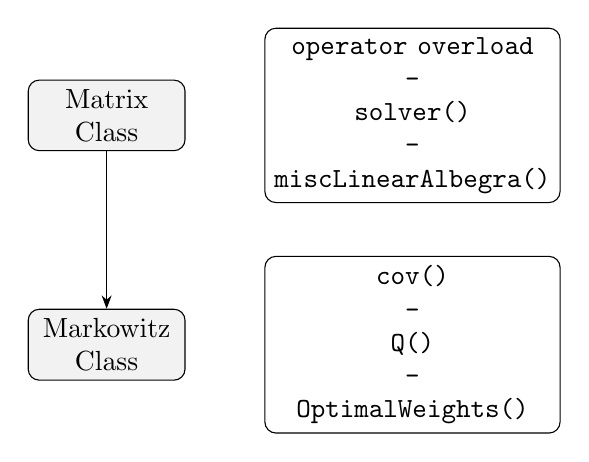
\begin{tikzpicture}[
    class/.style={rectangle, draw=black, fill=gray!10, rounded corners, 
                  minimum height=2em, minimum width=5em, text centered, 
                  text width=5em},
    class box/.style={rectangle, draw=black, fill=white, rounded corners, 
                      minimum height=2em, minimum width=10em, text centered, 
                      text width=10em, font=\ttfamily},
    relation/.style={-{Stealth}, thin}
]

% Define classes
\node[class] (class1) {Matrix Class};
\node[class, below=of class1, yshift=-1cm] (class2) {Markowitz Class};

% Class contents
\node[class box, right=of class1] (class1Methods) {operator overload \\ - \\ solver() \\ - \\miscLinearAlbegra()};

\node[class box, right=of class2] (class2Methods) {cov() \\ - \\ Q() \\ - \\ OptimalWeights()};



% Relations
\draw[relation] (class1) -- (class2);

\end{tikzpicture}

% Sequence Diagram
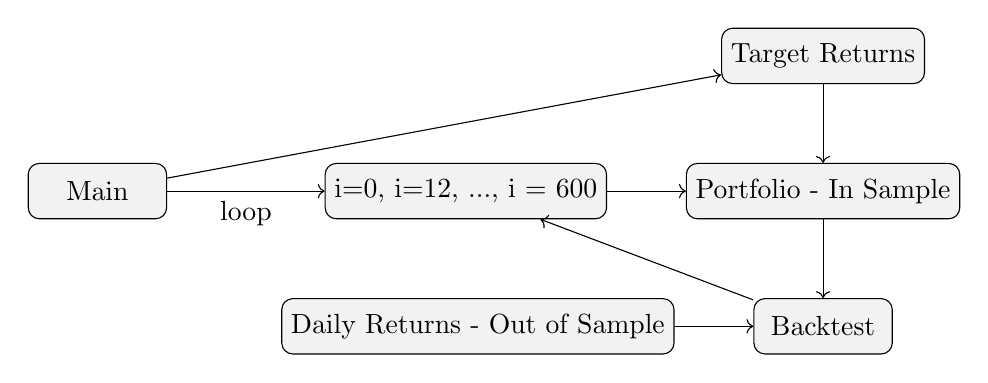
\begin{tikzpicture}[
    actor/.style={rectangle, draw=black, fill=gray!10, rounded corners, 
                  minimum height=2em, minimum width=5em, text centered},
    message/.style={->, thin}
]

% Actors and Objects
\node[actor] (user) {Main};
\node[actor, right=of user, xshift=1cm] (system) {i=0, i=12, ..., i = 600};
\node[actor, right=of system] (third) {Portfolio - In Sample};
\node[actor, below=of third] (fourth) {Backtest};
\node[actor, left=of fourth] (fifth) {Daily Returns - Out of Sample};
\node[actor, above=of third] (sixth) {Target Returns};

% Messages
\draw[message] (user) -- node[below] {loop} (system);
\draw[message] (system) -- node[] {} (third);
\draw[message] (third) -- node[] {} (fourth);
\draw[message] (fifth) -- node[] {} (fourth);
\draw[message] (fourth) -- node[] {} (system);
\draw[message] (sixth) -- node[] {} (third);
\draw[message] (user) -- node[] {} (sixth);

\end{tikzpicture}

\section{Evaluation}

\begin{figure}[htbp!]
\centering % this centers the figure
\includegraphics[width = 1.0\hsize]{./figures/Realised_Rolling_Window_Average_OOS_Return_cpp.png} % span 1.0 times the horizontal size of the page
\caption{Realised Rolling Window Average OOS Return for each Target} 
\label{fig:OOS_rets}
\end{figure}


Fig.~\ref{fig:OOS_rets} portrays the rolling window realised average return for each target over the course of the backtest. There are 50 periods in the backtest, indexed on the x-axis of the plot. Out of Sample performance of the Markowtiz model is poor. The cumulative performance over the enitre domain is worse the larger the target return becomes. 


In evaluating the accuracy of our Markowitz implementation, we compare with a quick numpy implementation in python, where the use of the linalg library provides a relaible yardstick with which to measure the accuracy of the CGD solver in cpp. Fig.~\ref{fig:OOS_rets_python} shows the drastic impact of the fractional differences in optimal weights we see whilst solving with CGD, on the overall performance during the backtesting phase.


In both cases, the Markowitz portfolio effectively captures the market Beta, and produces returns consistent with the amount of risk taken by the investor (where the magnitude and direction of those returns are dictated by those of the market). 

\begin{figure}[]
\centering % this centers the figure
\includegraphics[width = 1.0\hsize]{./figures/Realised_Rolling_Window_Average_OOS_Return.png} % span 1.0 times the horizontal size of the page
\caption{Realised Rolling Window Average OOS Return for each Target - Python} 
\label{fig:OOS_rets_python}
\end{figure}

\begin{figure}[]
\centering % this centers the figure
\includegraphics[width = 1.0\hsize]{./figures/efficint_frontier.png} % span 1.0 times the horizontal size of the page
    \caption{} 
\label{fig:efficint_frontier}
\end{figure}

\begin{figure}[]
\centering % this centers the figure
\includegraphics[width = 1.0\hsize]{./figures/Cumulative_Rets.png} % span 1.0 times the horizontal size of the page
\caption{} 
\label{fig:Cumulative_Rets}
\end{figure}

\end{document}


\section{Introduction}
This is a template for coursework submission. Many macros and definitions can be found in \texttt{notation.tex}. This document is not an introduction to LaTeX. General advice if get stuck: Use your favorite search engine. A great source is also \mbox{\url{https://en.wikibooks.org/wiki/LaTeX}}.

\section{Basics}

\subsection{Figures}
A figure can be included as follows:
\begin{figure}[tb]
\centering % this centers the figure
\includegraphics[width = 0.7\hsize]{./figures/imperial} % this includes the figure and specifies that it should span 0.7 times the horizontal size of the page
\caption{This is a figure.} % caption of the figure
\label{fig:imperial figure} % a label. When we refer to this label from the text, the figure number is included automatically
\end{figure}
Fig.~\ref{fig:imperial figure} shows the Imperial College logo. 

Some guidelines:
\begin{itemize}
\item Always use vector graphics (scale free)
\item In graphs, label the axes
\item Make sure the font size (labels, axes) is sufficiently large
\item When using colors, avoid red and green together (color blindness)
\item Use different line styles (solid, dashed, dotted etc.) and different markers to make it easier to distinguish between lines
\end{itemize}

\subsection{Notation}
\begin{table}[tb]
\caption{Notation}
\label{tab:notation}
\centering
\begin{tabular}{ll}
Scalars & $x$\\
Vectors & $\vec x$\\
Matrices & $\mat X$\\
Transpose & $\T$\\
Inverse & $\inv$\\
Real numbers & $\R$\\
Expected values & $\E$\\
\end{tabular}
\end{table}
Table~\ref{tab:notation} lists some notation with some useful shortcuts (see latex source code).

\subsubsection{Equations}
Here are a few guidelines regarding equations
\begin{itemize}
\item Please use the \texttt{align} environment for equations (\texttt{eqnarray} is buggy)
\item Please number all equations: It will make things easier when we need to refer to equation numbers. If you always use the \texttt{align} environment, equations are numbered by default.
\item Vectors are by default column vectors, and we write 
\begin{align}
\vec x &= \colvec{1,2}
\end{align}
\item Note that the same macro (\texttt{$\backslash$colvec}) can produce vectors of variable lengths, as
\begin{align}
\vec y &= \colvec{1,2,3,4}
\end{align}
\item Matrices can be created with the same command. The \& switches to the next column:
\begin{align}
\mat A = \begin{bmatrix}
1 & 2 & 3\\
3 & 4 & 5
\end{bmatrix}
\end{align}
\item Determinants. We provide a simple macro (\texttt{$\backslash$matdet}) whose argument is just a matrix array:
\begin{align}
\matdet{
1 & 2 & 3\\
3 & 4 & 5\\
2 & 2 & 2
}
\end{align}
\item If you do longer manipulations, please explain what you are doing: Try to avoid sequences of equations without text breaking up. Here is an example:
We consider
\begin{align}
U_1 = [\colvec{1,1,0,0},\, \colvec{0,1,1,0},\, \colvec{0,0,1,1}]
\subset\R^4, \quad 
U_2 = [\colvec{-1,1,2,0},\, \colvec{0,1,0,0}]
\subset\R^4\,.
\end{align}
To find a basis of $U_1\cap U_2$, we need to find all $\vec x \in V$ that can be represented as linear combinations of the basis vectors of $U_1$ and $U_2$, i.e., 
\begin{align}
\sum_{i=1}^3 \lambda_i \vec b_i = \vec x = \sum_{j=1}^2 \psi_j \vec c_j\,,
\end{align}
where $\vec b_i$ and $\vec c_j$ are the basis vectors of $U_1$ and $U_2$, respectively.
%
The matrix $\mat A = [\vec b_1|\vec b_2|\vec b_3| -\vec c_1|-\vec
c_2]$ is given as
\begin{align}
\mat A = 
\begin{bmatrix}
1 & 0 & 0 & 1 & 0\\
1 & 1 & 0 & -1 & -1\\
0 & 1 & 1 & -2 & 0\\
0 & 0 & 1 & 0 & 0
\end{bmatrix}\,.
\end{align}
By using Gaussian elimination, we determine the corresponding reduced row echelon form 
\begin{align}
\begin{bmatrix}
1 & 0 & 0 & 1& 0\\
0 & 1 & 0 & -2 & 0\\
0 & 0 & 1 & 0 & 0\\
0 & 0 & 0 & 0 & 1
\end{bmatrix}
\,.
\end{align}
We keep in mind that we are interested in finding $\lambda_1,\lambda_2,\lambda_3\in\R$ and/or $\psi_1,\psi_2\in\R$ with 
\begin{align}
\begin{bmatrix}
1 & 0 & 0 & 1& 0\\
0 & 1 & 0 & -2 & 0\\
0 & 0 & 1 & 0 & 0\\
0 & 0 & 0 & 0 & 1
\end{bmatrix}
\colvec{\lambda_1, \lambda_2, \lambda_3, \psi_1, \psi_2}
=\vec 0\,.
\end{align}
From here, we can immediately see that $\psi_2=0$ and $\psi_1\in\R$ is
a free variable since it corresponds to a non-pivot column, and our solution is 
\begin{align}
U_1\cap U_2 = \psi_1\vec c_1 =  [ \colvec{-1,1,2,0} ]
\,, \quad \psi_1\in\R\,.
\end{align}
\end{itemize}


\subsection{Gaussian elimination}
We provide a template for Gaussian elimination. It is not perfect, but it may be useful:

\begin{elimination}[6]{5}{8mm}{1}
    \eliminationstep
        {
        1 & - 2 & 1 & -1 & 1 &  0\\     
        0 & 0 & -1 & 1 & -3 & 2\\
        0 & 0 & 0 & -3 & 6 & -3\\
        0 & 0 & -1 & -2 & 3 & a
            }
                {
                \\
                \\
                \\
                -R_2
                    }
                        \\
                        \eliminationstep
                         {
                         1 & - 2 & 1 & -1 & 1 &  0\\     
                         0 & 0 & -1 & 1 & -3 & 2\\
                         0 & 0 & 0 & -3 & 6 & -3\\
                         0 & 0 & 0 & -3 & 6 & a-2
                             }
                                 {
                                 \\
                                 \\
                                 \\
                                 -R_3
                                     }\\
                                     \eliminationstep{
                                     1 & - 2 & 1 & -1 & 1 &  0\\     
                                     0 & 0 & -1 & 1 & -3 & 2\\
                                     0 & 0 & 0 & -3 & 6 & -3\\
                                     0 & 0 & 0 & 0 & 0 & a+1
                                     }
                                     {
                                     \\
                                     \cdot (-1)\\
                                     \cdot (-\tfrac{1}{3})\\
                                     \\}
                                     \\
                                     \eliminationstep{
                                     1 & - 2 & 1 & -1 & 1 &  0\\     
                                     0 & 0 & 1 & -1 & 3 & -2\\
                                     0 & 0 & 0 & 1 & -2 & 1\\
                                     0 & 0 & 0 & 0 & 0 & a+1
                                     }{}
                                     \end{elimination}

                                     The arguments of this environment are:
                                     \begin{enumerate}
                                     \item Number of columns (in the augmented matrix)
                                     \item Number of free variables (equals the number of columns after which the vertical line is drawn)
                                     \item Column width
                                     \item Stretch factor, which can stretch the rows further apart.
                                     \end{enumerate}



                                     \newpage
                                     \section{Answer Template}
                                     \begin{enumerate}[1)]
                                     \item Discrete models

                                     \begin{enumerate}[a)]
                                     \addtocounter{enumii}{2} % change to enumi if you use sections rather than enumerate for question numbers
                                     \item 
                                     \item
                                     \item 
                                     \end{enumerate}


                                     \item Differentiation

                                     \begin{enumerate}[a)]
                                     \item 
                                     \item
                                     \addtocounter{enumii}{1} 
                                     \item 
                                     \item
                                     \end{enumerate}


                                     \item Continuous Models

                                     \begin{enumerate}[a)]
                                     \item 
                                     \item
                                     \item 
                                     \item 
                                     \item
                                     \item 
                                     \item 
                                     \end{enumerate}

                                     \item Linear Regression


                                     \begin{enumerate}[a)]
                                     \item 
                                     \item
                                     \item 
                                     \item 
                                     \end{enumerate}

                                     \item Ridge Regression


                                     \begin{enumerate}[a)]
                                     \item 
                                     \item
                                     \item 

                                     \begin{enumerate}[i)]
                                     \item 
                                     \item
                                     \end{enumerate}

                                     \end{enumerate}

                                     \item Bayesian Linear Regression


                                     \begin{enumerate}[a)]
                                     \addtocounter{enumii}{1} 
                                     \item 
                                     \item
                                     \item 
                                     \item (bonus)
                                     \end{enumerate}

                                     \end{enumerate}














                                     \end{document}
                                     %%% Local Variables: 
                                     %%% mode: latex
                                     %%% TeX-master: t
                                     %%% End: 

